\section{Inflasjon}
Inflasjon er nødvendig å ta hensyn til ettersom pengeverdien i en flerperiodisk analyse vil forandre seg over tid. Å gi et korrekt anslag av hvordan dette vil utvikle seg i årene fremover er vanskelig på grunn av usikkerhet i markedet, men vi legger til grunn prognoser fra Norges Bank som anslår en fremtidig inflasjons økning på 2\%. Tolvmånedersendringen (Mars 2018- Mars 2019) ligger på 2,9\%, men er ventet å synke de kommende årene \cite{inflasjon}.

\section{Utvikling i norsk økonomi}
Norsk økonomi er inne i en oppgangskonjunktur. I 2018 var BNP-veksten 1,4\%, og det forventes at veksten i 2019 vil øke til 2,3\% basert på forrige år. Bakgrunnen for de gode tallene er økt sysselsetting, høy aktivitet i flere bransjer og investeringene i fastlandsbedriftene har ikke vært høyere på 10 år. I motsetning til Norge har veksten i flere land i Europa avtatt den siste tiden, noe som kan føre til lavere etterspørsel etter norske varer. 

\indent \newline
Økte boligpriser har gjort boligbygging mer lønnsomt de siste årene. Dersom oppgangskonjunkturen i Norge fortsetter, noe som bidrar til økte inntekter, kan dette tale for enda flere boligutbyggelser. Derimot taler renteheving og lavere befolkningsvekst mot dette. Dette gir grunn til å anslå den fremtidige veksten i bygg- og anleggsbransjen til å være relativt moderat \cite{norskokonomi}.

\section{Økende fokus på miljø}
De siste årene har fokus på miljø blitt viktigere, både på et globalt- og nasjonalt nivå. I 2015 vedtok medlemslandene i FN 17 mål for bærekraftig utvikling som varer frem til 2030. Flere av målene omhandler å bekjempe klimaendringene og konsekvensene av dem. Dette gjelder spesielt reduksjon i utslipp av klimagasser. Der mange virksomheter tidligere ikke har måtte ta hensyn til utslipp og bærekraftig produksjon, har dette blitt en viktig del av hverdagen, og spesielt fremtiden. I tillegg til å jobbe mot FNs bærekraftsmål har Norge forpliktet seg til å oppfylle Parisavtalen. På bakgrunn av dette stilles det strengere krav til norske virksomheters CO2-fotavtrykk i form av både utslipp og avfall (deponi). Det forventes at kravene vil øke med tiden \cite{baerekraftsmaal}.

\subsection{Klimakvoter}
Klimakvoter er tillatelser til å slippe ut en viss mengde klimagasser. Disse blir som regel målt i tonn. Norge har gjennom EØS-avtalen vært en del av Det europeiske kvotesystemet siden 2008. I et kvotesystem finnes det et bestemt antall kvoter som kan selges og kjøpes. Antall tilgjengelige kvoter reduseres over tid med et formål om å kutte totalutslippet av klimagasser. Det europeiske kvotesystemet omfatter om lag 140 norske virksomheter innenfor industrier som gass- og kullkraftverk, energianlegg, petroleumsutvinning og offshoreanlegg, raffinerier, treforedling, jern- og stålproduksjon, ferrolegeringer, aluminium, mineralgjødsel, sement og kalk. Norge og EU har gjennom Paris-avtalen forpliktet seg til å redusere klimautslippene med minst 40 prosent regnet fra 1990 til 2030, og redusere utslippene i det europeiske kvotesystemet med 43 prosent fra 2005 til 2030.

\indent \newline
Reduksjonen foregår ved å senke taket på det totale antall kvoter i systemet. Knapphet på kvoter skaper dermed en markedspris på utslippene, hvor en høyere pris skaper insentiv til å redusere utslippene. I praksis kan en virksomhet som klarer å redusere utslipp til et nivå som gir dem et overskudd av kvoter selge disse til andre virksomheter som ligger på et høyere nivå enn tildelte kvoter. Fra 2010 har nedskaleringsfaktoren ligget på 1,74 prosent og vil gjelde ut 2020. Fra og med 2021 vil faktoren øke til 2,2 prosent per år og dermed skape større press på de kvotepliktige virksomhetene til å kutte utslipp \cite{klimakvoter}.

\indent \newline
Antall tilgjengelige kvoter i systemet påvirker prisen per kvote. Fra 2010 frem til 2018 har prisen omtrent ligget mellom 5 og 15 euro. Imidlertid har prisen økt kraftig de to siste årene og ligger per mai 2019 på 25 euro. Den kraftige økningen er ventet å fortsette, spesielt i årene etter 2021 hvor den nye nedskaleringsfaktoren tas i bruk \cite{kvotemarked}.
Figuren under viser rockwool sitt co2-utslipp (rød graf) og tildelte kvoter (grønn graf) i perioden 2012-2017.

\begin{figure}[H]
  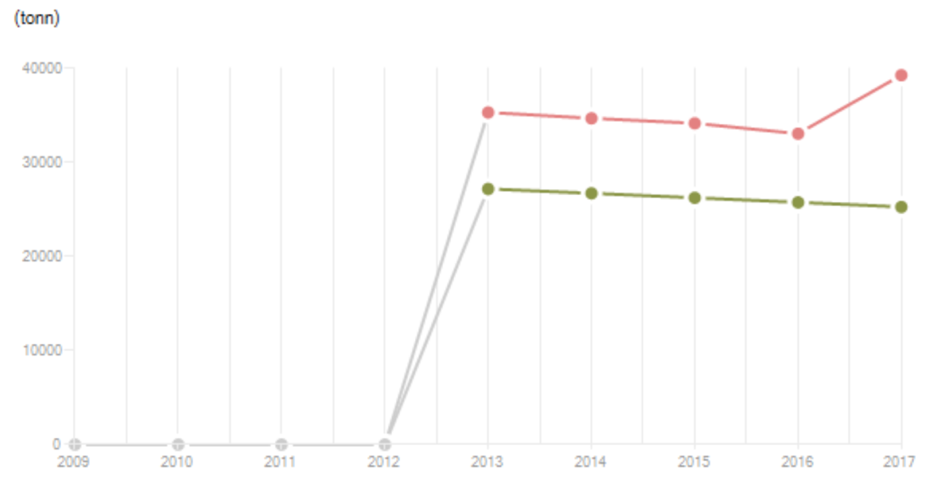
\includegraphics[width=\linewidth]{bilder/co2utslipp.png}
  \caption{Rockwool kvote og co2-utslipp - \cite{utslippkvote}}
  \label{fig:co2utslipp}
\end{figure}

\subsection{Avfall/resirkulering}
I 2015 presenterte Europakommisjonen et forslag til en ny sirkulær-økonomi pakke som blant annet omhandler endring av avfalls - og resirkuleringsregelverket. Målet med forslaget er å bedre den miljømessige samfunnsutviklingen gjennom effektivisering av ressursbruk gjennom hele verdikjeden (produksjon, forbruk og avfallsbehandling). En sirkulær økonomi er basert på gjenbruk, reparasjon, oppussing/forbedring og materialgjenvinning hvor færrest mulig ressurser går tapt \cite{sirkularokonomi}.

\indent \newline
Videre ble det i 2018 vedtatt endringer i deponidirektivet som er en del av sirkulær-økonomi pakken. Endringene omhandler strengere krav og begrensninger på avfall som tillates deponert. Dette gjelder spesielt avfall som egner seg for materialgjenvinning \cite{materialgjenvinning}.

\section{Kraftpriser}
Den nye smelteovnen til Rockwool vil bruke elektrisitet som energikilde, noe som krever økt strømforbruk. I den forbindelse er det viktig å gjøre anslag om hvordan strømprisen kan endres gjennom investeringens levetid.

\indent \newline
Det er flere faktorer som ligger til grunn for strømprisen i Norge. De viktigste er værforholdet, etterspørsel, kull- og gasspriser og prisen på CO2-kvoter. Norge er koblet opp mot det Europeiske kraftmarkedet, noe som fører til at svingninger i pris og produksjon i utlandet vil påvirke prisene i Norge. Krafthandlene gjøres gjennom Nord Pool AS, et aksjeselskap som eies av de nordiske og baltiske stamnettoperatørene.

\indent \newline
Været er den største forklaringskraften på hvor mye strøm Norge produserer hvert år. Basert på at omtrent 95\% av produsert elektrisitet kommer fra vannkraft vil nedbørsmengden ha stor innvirkning på eksport- og importbehovene til Norge. Anslag om fremtidige værutsikter er tilnærmet umulig, men man kan forutse en endring i klima basert på global oppvarming. Effekten av dette vil være vanskelig å forutse.

\indent \newline
Det er spådd en økning i etterspørselen etter elektrisitet i industri- og kraftmarkedet i fremtiden. Prognoser fra NVE (Norges Vassdrags- og Energidirektorat) viser til at norsk
industri kommer til å øke strømforbruket med omtrent 28\% fra 2018 til 2040. Dette
begrunnes med en økning i antall datasentre, og at flere industrier vil rette et større fokus mot en miljørettet profil.

\indent \newline
Ettersom Norge er koblet mot det Europeiske kraftmarkedet vil priser på kull og gass ha innvirkning på strømprisen i Norge. Store deler av produksjonen i Europa er preget av kullkraft, noe som betyr at en økning i kullprisen kan minske produksjonen i kullkraftverkene. Dette vil resultere i lavere kraftproduksjon, altså lavere tilbud, og økte priser. Det samme resonnementet gjelder CO2-kvoter.

\indent \newline
Historiske tall viser at strømprisen er relativt volatil. NVE estimerer fremtidig spotpris til mellom 36-37 øre pr kWh (Kilowattime) frem til 2030. Normalt vil det tillegges el-avgift og MVA på denne prisen. Relevant sats for disse er henholdsvis 0,48 øre per kWh for el-avgiften og MVA-satsen er på 25\%. El-avgiften for husholdninger er dog høyere, men industrinæringer har redusert sats.

\begin{table}[H]
  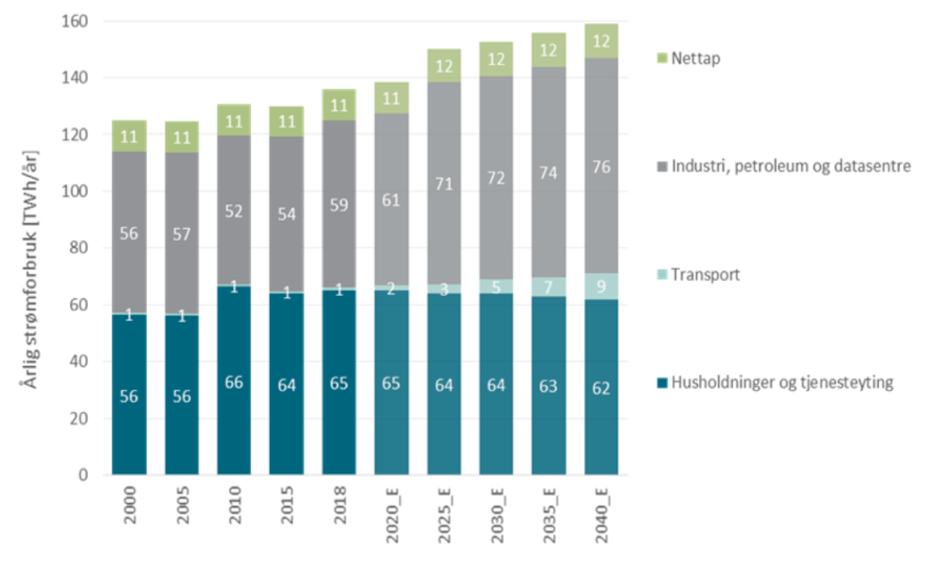
\includegraphics[width=\linewidth]{tabeller/stromforbruk.png}
  \caption{Strømforbruk - utvikling}
  \label{tbl:stromforbruk}
\end{table}

\begin{figure}[H]
  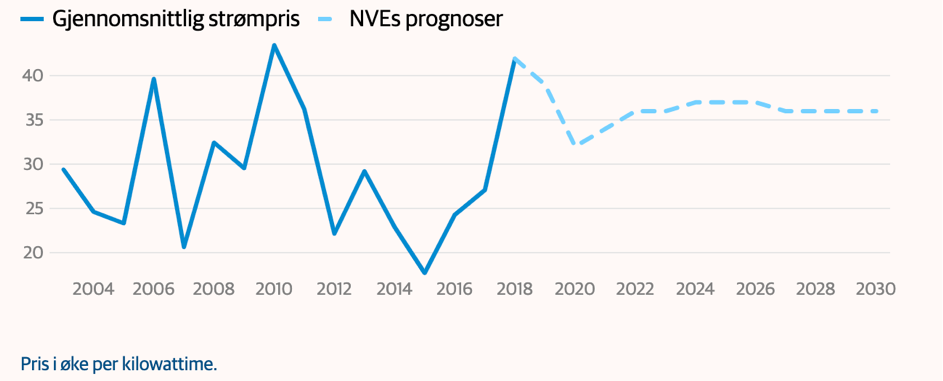
\includegraphics[width=\linewidth]{bilder/strompris.png}
  \caption{Strømpris - utvikling}
  \label{fig:strompris}
\end{figure}



 